\section{Simulation}

In this section simulation results will be presented and analysed. Simulations are conducted in the Gazebo simulator within the ROS environment. UAV used in experiments is the $\mu$Morus with moving-masses which can be found in the \textit{mmuav\_gazebo} repository \cite{gitLink}, along with its parameters. 
Control parameters are chosen as follows:
\begin{equation*}
	k_x = 
	\begin{bmatrix}
		10 &  0  &  0 \\
		 0 & 10  &	0 \\ 
		 0 &  0  & 50 	
	\end{bmatrix}
	\, , \,	
	k_v =
	\begin{bmatrix}
		3.75 & 0 & 0 \\
		0 & 3.75 & 0 \\
		0 & 0 & 20
	\end{bmatrix}
\end{equation*}
\begin{equation*}
	k_R = 
	\begin{bmatrix}
		1.5 & 0 & 0 \\
		0 & 1.5 & 0 \\
		0 & 0 & 10
	\end{bmatrix}
	\, , \,
	k_\Omega = 
	\begin{bmatrix}
		0.65 & 0 & 0 \\
		0 & 0.65 & 0 \\
		0 & 0 & 1.54
	\end{bmatrix}
\end{equation*}

It is important to note that the actuator dynamics of the moving masses is taken in consideration within the Gazebo simulation environment. Furthermore there is a slight transient delay when increasing or decreasing rotor velocity which results in a non-instantaneous control force change. These phenomena were not taken in consideration while modeling the system and choosing control terms. \\

The chosen trajectory tracking problem is formulated as a 20 second rotating spiral:
\begin{gather*}
	\vec{x}_d(t) = [0.4\text{t}; \, 0.5\text{sin}(\pi\text{t}); \, 0.6\text{cos}(\pi\text{t}) + 2] \\
	\vec{b}_{1,d}(t) = [\text{cos}\left(\frac{\pi}{5}\text{t}\right); \, \text{sin}\left(\frac{\pi}{5}\text{t}\right); \, 0]
\end{gather*}

\noindent Initial position and orientation is chosen at the start of the trajectory.

\newpage
\begin{figure}[h!]
	\centering
	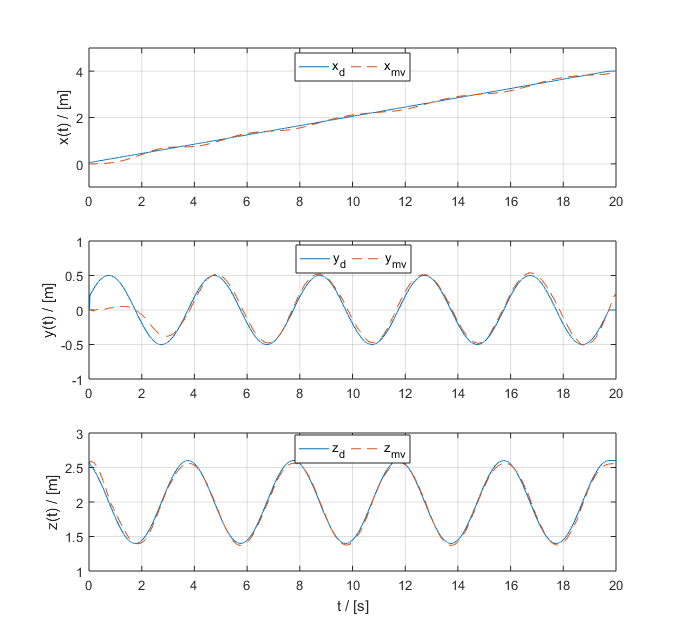
\includegraphics[width=\columnwidth]{./pictures/mmc_traj_pos.png}
	\caption{Comparison of the desired $\vec{x}_d$ and measured position values $\vec{x}_{mv}$.}
	\label{fig:traj_pos}
\end{figure}

\begin{figure}[h!]
	\centering
	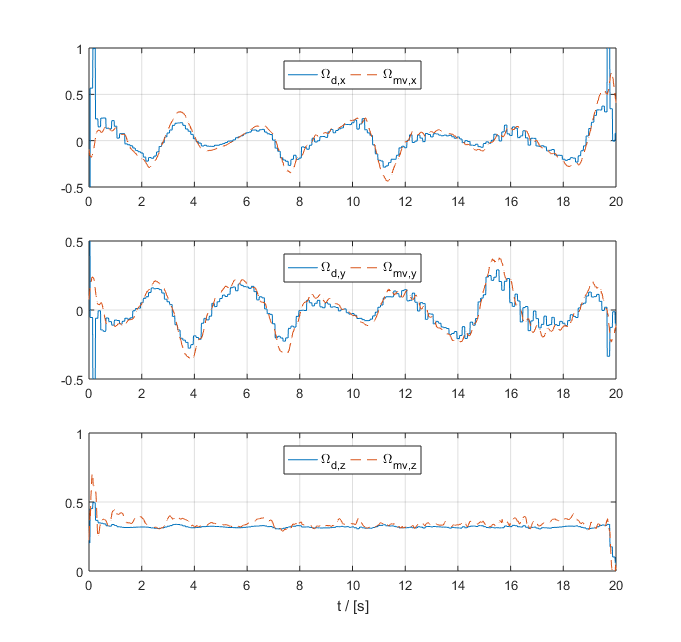
\includegraphics[width=\columnwidth]{./pictures/mmc_traj_omega.png}
	\caption{Comparison of desired $\Omega_d$ and measured $\Omega_{mv}$ angular velocity values.}
	\label{fig:traj_omega}
\end{figure}

\begin{figure}[h!]
	\centering
	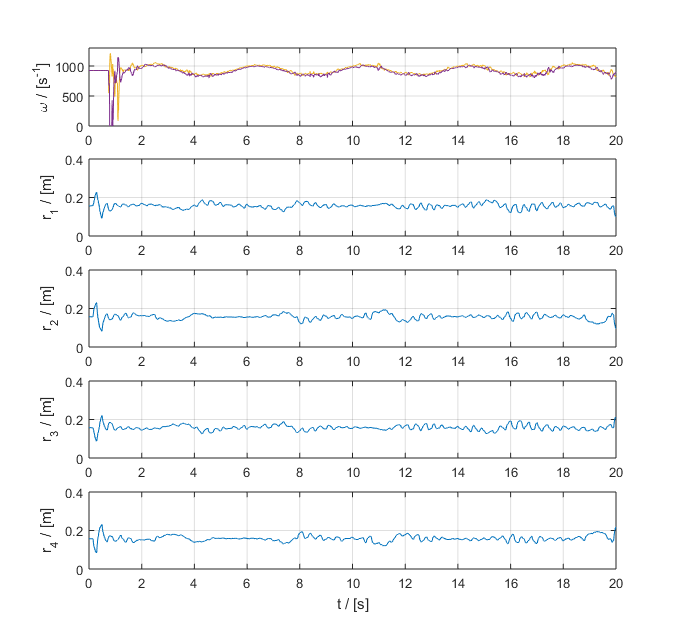
\includegraphics[width=\columnwidth]{./pictures/mmc_traj_rotorVel_massOff.png}
	\caption{Display of all control inputs: rotor velocities $\omega_i$ and mass offsets $r_i$ along $\vec{b}_{1,d}$ and $\vec{b}_{2,d}$ body-fixed frame axis.}
	\label{fig:rotorVel_massOff}
\end{figure}

\begin{figure}[h!]
	\centering
	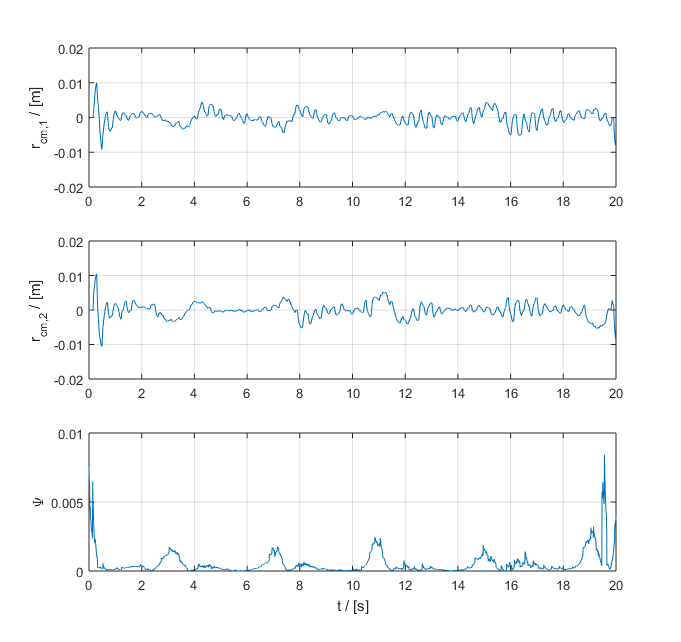
\includegraphics[width=\columnwidth]{./pictures/mmc_traj_rCm_attErr.png}
	\caption{First two components of CoG vector $\vec{r}_{CoG}$ (third component is always zero since masses only move in x-y plane of the body-fixed frame) and attitude error function $\Psi$. }
	\label{fig:rCm_attErr}
\end{figure}
